\begin{prob}
    Draw a directed graph with three nodes $u,v,w$ such that: 1) $v$ is
    reachable from $u$; 2) in a DFS started at $w$, the finish time of $v$
    is larger than the finish time of node~$u$.

    \begin{soln}
        Consider this graph:

        \begin{center}
            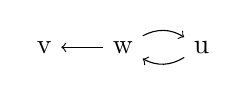
\begin{tikzpicture}
                \node (v) at (0,0) {v};
                \node (w) at (1,0) {w};
                \node (u) at (2,0) {u};

                \draw (w) edge[->] (v);
                \draw (w) edge[->, bend left] (u);
                \draw (u) edge[->, bend left] (w);
            \end{tikzpicture}
        \end{center}

        Start a DFS at node $w$. The DFS will then visit node $u$, then
        node $v$. The finish time of node $u$ will be 2, while the finish time
        of node $v$ will be 5. But $v$ is reachable from $u$.
    \end{soln}

\end{prob}
